\documentclass[10pt,a4paper]{article}
\usepackage[ngerman,english]{babel}
\usepackage[utf8]{inputenc}
\usepackage{hyperref}
\usepackage{graphicx}
\usepackage{algpseudocode}
\usepackage{amssymb}
\usepackage{amsmath}
\usepackage{amsthm}
\usepackage{listings}
\title{Polytopes}
\author{Henrique Hepp, ...}
\newcommand{\Tau}{\mathcal{T}} 
\newtheorem{thm}{Theorem}
\begin{document}
\maketitle

\section{Introduction}

\begin{thm}[Steinitz, 1922]
A graph G is the edge graph of a 3-polytope if
and only if G is simple, planar and 3-connected.
\end{thm}

\section{Equilibrium Stresses}

\begin{thm}[Maxwell, Whiteley]
Let G be a planar 3-connected graph with 2D drawing $\mathbf{p}$ and designated outer face $f_0$ . There exists a one-to-one correspondence between
\begin{enumerate}
\item equilibrium stresses $w$ for $G$ at $\mathbf{p}$; and
\item liftings in $\mathbb{R}$ , where face $f_0$ remains in the $z = 0$ plane.
\end{enumerate}

\end{thm}


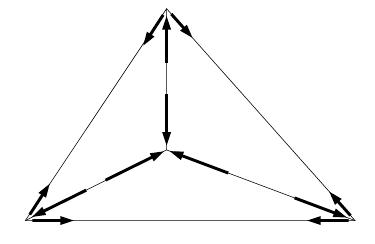
\includegraphics[scale=0.8]{stresses.png} 

\section{The algorithms}

The algorithm based on the article ``Embedding Stacked Polytopes on a Polynomial-Size Grid'' 2011 can be divided in:

\begin{enumerate}
\item Receive the entry.
\item Heavy caterpillar decomposition.
\item Balance the tree.
\item Get the coefficients, or weights for the lifting.
\item Lift the graph to a polytope. 
\end{enumerate}

The algorithm presented in the definitives version was changed in the two last topics. It can be divided in:

\begin{enumerate}
\item Receive the entry.
\item Heavy caterpillar decomposition.
\item Balance the tree.
\item Lift the graph to a polytope. 
\item Round the graph to grid points.
\end{enumerate}
 

\section{The Entry of the algorithm}

It is given to the algorithm a 3 connected planar graph and a tree representation of the graph, as showed below.

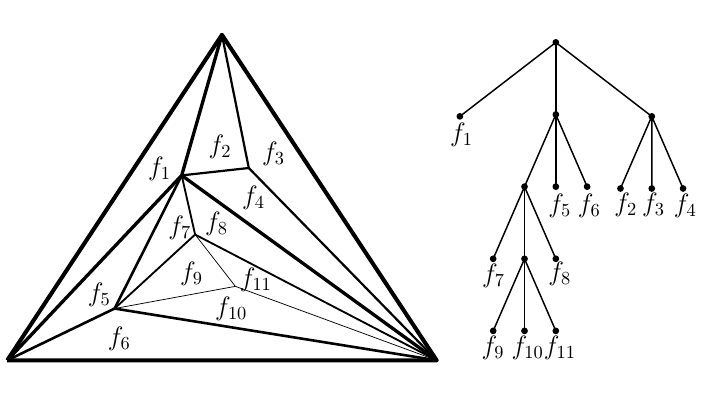
\includegraphics[scale=0.8]{graph_tree.png} 

\section{Heavy caterpillar decomposition}
The tree representation is decomposed in \textit{heavy paths}. Resulting sub-trees called \textit{caterpillars}. When a node lies on a heavy path it is called a \textit{spine node}, otherwise is a \textit{tree node}. The spine nodes are labelled by $s_1$ (root), $s_2$, ..., $s_i$,...,$s_\bot$. The children from $s_i$ are $s_{i+1}$, $t_{i+1}$ and $t'_{i+1}$. In $t$ are stored a pointer link$(t)$ to a other caterpillar. 

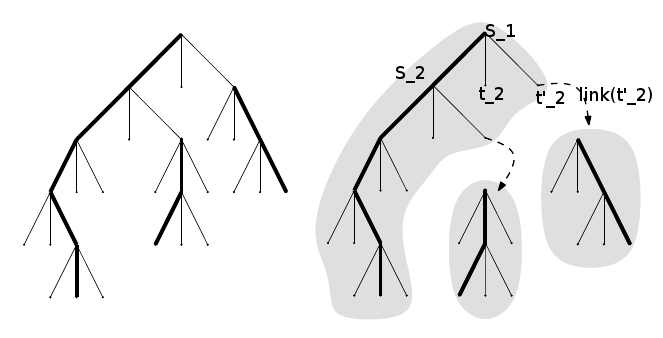
\includegraphics[scale=1]{caterpillarEdit.png} 

\section{Balance the tree}


The balacing of the Tree is given by the pseudo-code below:

\begin{algorithmic}
\Function{BALANCE}{C} 
\State \textbf{Input:} A caterpillar $C$ from the heavy caterpillar decomposition of $\Tau(G)$. All weights are equal 1.
\State \textbf{Output:} Weights for the nodes of $\Tau(G)$.

\ForAll{$t_i$, $t'_i$ in $C$} 
	\State BALANCE(link($t_i$))
	\State BALANCE(link($t'_i$))
    \If {$w(t_i)>w(t'_i)$}
        \State relabel $t_i \leftrightarrow t'_i$
    \EndIf
	\State $w(t_i)=w(t'_i)$
	\State add $(w(t_i ) - w(t'_i ))$ to the weight of $s_{\bot}$ in link $(t_i)$
	\State add $(w(t'_i ) - w(t_i ))$ to the weight of link$^{-1} (C)$
\EndFor
\EndFunction
\end{algorithmic}


A balanced Tree will the have the properties:

$$w(s_{i-1})= w(s_i) + w(t_i) + w(t'_i)$$

$$w(s_i)\geq w(t_i),w(t'_i) $$

$$w(t_i)= w(t'_i) $$

A example of a balanced tree is show next: 

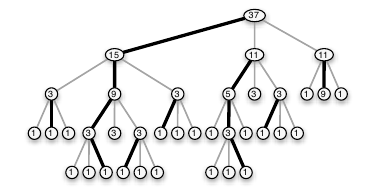
\includegraphics[scale=1]{balancedTree.png} 


\section{First algorithm}

\subsection{Get the coefficients}

If $v_i$ is the vertex stacked on the face $v_jv_kv_l$ then:

$$\alpha_{ijkl} = \frac{1}{w(t_u)}$$

Where $w(t_u)$ is the weight of the subface $v_jv_kv_l$ obtained by the function BALANCE.

The weights are now updated with the coordinate values. First the coordinates from the vertices are rounded down. $r_i = (\lfloor x_i \rfloor, \lfloor y_i\rfloor)$.

The weights are:

$$\dot{w}_{ij}= \sum_{\{i,j,k,l\}\in S} \lfloor Y \alpha_{ijkl}\rfloor w^{kl}_{ij}$$   

\textit{I have to find out how to make that sum}

The coefficient $\alpha_{ijkl}$ is scaled by multiplying it with $Y = 4 n^2$, $n$ is the number of vertices.


$$w^{kl}_{ij}= [i,k,l][j,k,l]$$

$$
[i,j,k]= \text{det}
 \begin{pmatrix}
  x_i & x_j & x_k\\
  y_i & y_j & y_k\\
  1	  & 1   & 1  \\
 \end{pmatrix}
$$

\subsection{The lifting}

Each face $i$ gains a parameter $a_i$ in that way:

For the firs face is set:

$$a_0 = (0,0,0)^T$$   

Having the parameter of the rigth face (the first is $a_0$ ) then we can find all the others with:

$$a_l= \dot{w}_{ij}(\mathbf{q}_i\times\mathbf{q}_j)+a_r$$

Where $(i,j)$ is the common edge of $f_i$ and $f_l$ and $\mathbf{q}_i$ is defined as:

$$\mathbf{q}_i = (x_i,y_i,1)^T$$

Now to calculate the height from a point $\mathbf{p}_i$ we have to make the inner product from $\mathbf{p}_i$ with $a_k$. Who is the parameter from face $k$ whose one of the vertices is $\mathbf{p}_i$.

$$h_i = \langle \mathbf{p}_i, a_k\rangle$$

\section{Second algorithm}

\subsection{Calculate the shifts} 

As the vertex $v_i$ is stacked on a face $f_D$ is new height is:

$$z= \zeta_i + z_D $$

Where $z_D$ is the height of the point in the face $D$ and the shift $\zeta_i$ is:

$$\zeta_i = A_i\cdot B_i$$

Where  $ A_i$ and $B_i$ are the two possible weights of the three new faces formed by the vertex $v_i$. Remember $w(t_i)= w(t'_i) $.

But before we calculate the new heights ($z_i$) we round the coordinates in the embedding, and then also the heights.

\subsection{Round the graph to grid points}

The coordinates on the embedding are all rounded so that they are multiples of $1/\text{pert}$, where:

$$\text{pert}=240n^{\frac{3}{2}}$$

Now we lift, rounding, the points so that the heights $z= \zeta_i + z_D $ are multiples of $1/\text{pert}_z$, where: 

$$\text{pert}_z=3n$$ 

After these points are rounded they are still real numbers, not intengers. To make them integer we multiply they with pert.

To make the rounding we calculate:

$$\lfloor x\cdot\text{pert}\rfloor \div \text{pert}$$

The final value in integer is:

$$\lfloor x\cdot\text{pert}\rfloor \div \text{pert} \cdot\text{pert} = \lfloor x\cdot\text{pert}\rfloor$$

\end{document}
